\documentclass{beamer}
\usetheme{Berlin}
\usecolortheme{dolphin}

\usepackage[T1]{polski}
\usepackage[polish]{babel}
\usepackage[utf8]{inputenc}
\usepackage[T1]{fontenc}
\usepackage[mediumspace,mediumqspace,Grey,squaren]{SIunits}
\usepackage{graphicx}
\usepackage{hyperref}

%\addbibresource{bibliography.bib}

%\setbeamertemplate{bibliography item}{\insertbiblabel}


\graphicspath{ {./images/} }

\begin{document}
\title{Seminarium dyplomowe magisterskie}
\author{Jakub Postępski}
\date{29 listopada 2018}

\frame{\titlepage}

\section{Zarys pracy magisterskiej}
\begin{frame}{Sterowanie ramieniem robota w obliczu chwytania przedmiotów}

\begin{itemize}
\item Dr inż. Tomasz Winiarski
\end{itemize}

\begin{itemize}
\item Sterowanie siłowe
\item Odczyty wartości z efektorów i receptorów
\item Nieznany model chwytanego obiektu
\end{itemize}
\end{frame}

\section{Środowisko badawcze}

\begin{frame}{Robot usługowy Velma}
\begin{itemize}
\item Dwa manipulatory LWR (sterowanie impedancyjne)
\item Chwytaki Barretta (sztuczna skóra, czujniki siły)
\item Nadgarstkowe czujniki siły i momentu
\item Kinect
\item Stereopara
\item Komputer sterujący
\end{itemize}
\end{frame}

\begin{frame}{Zdjęcie robota Velma}
\begin{figure}[h]
	\centering
	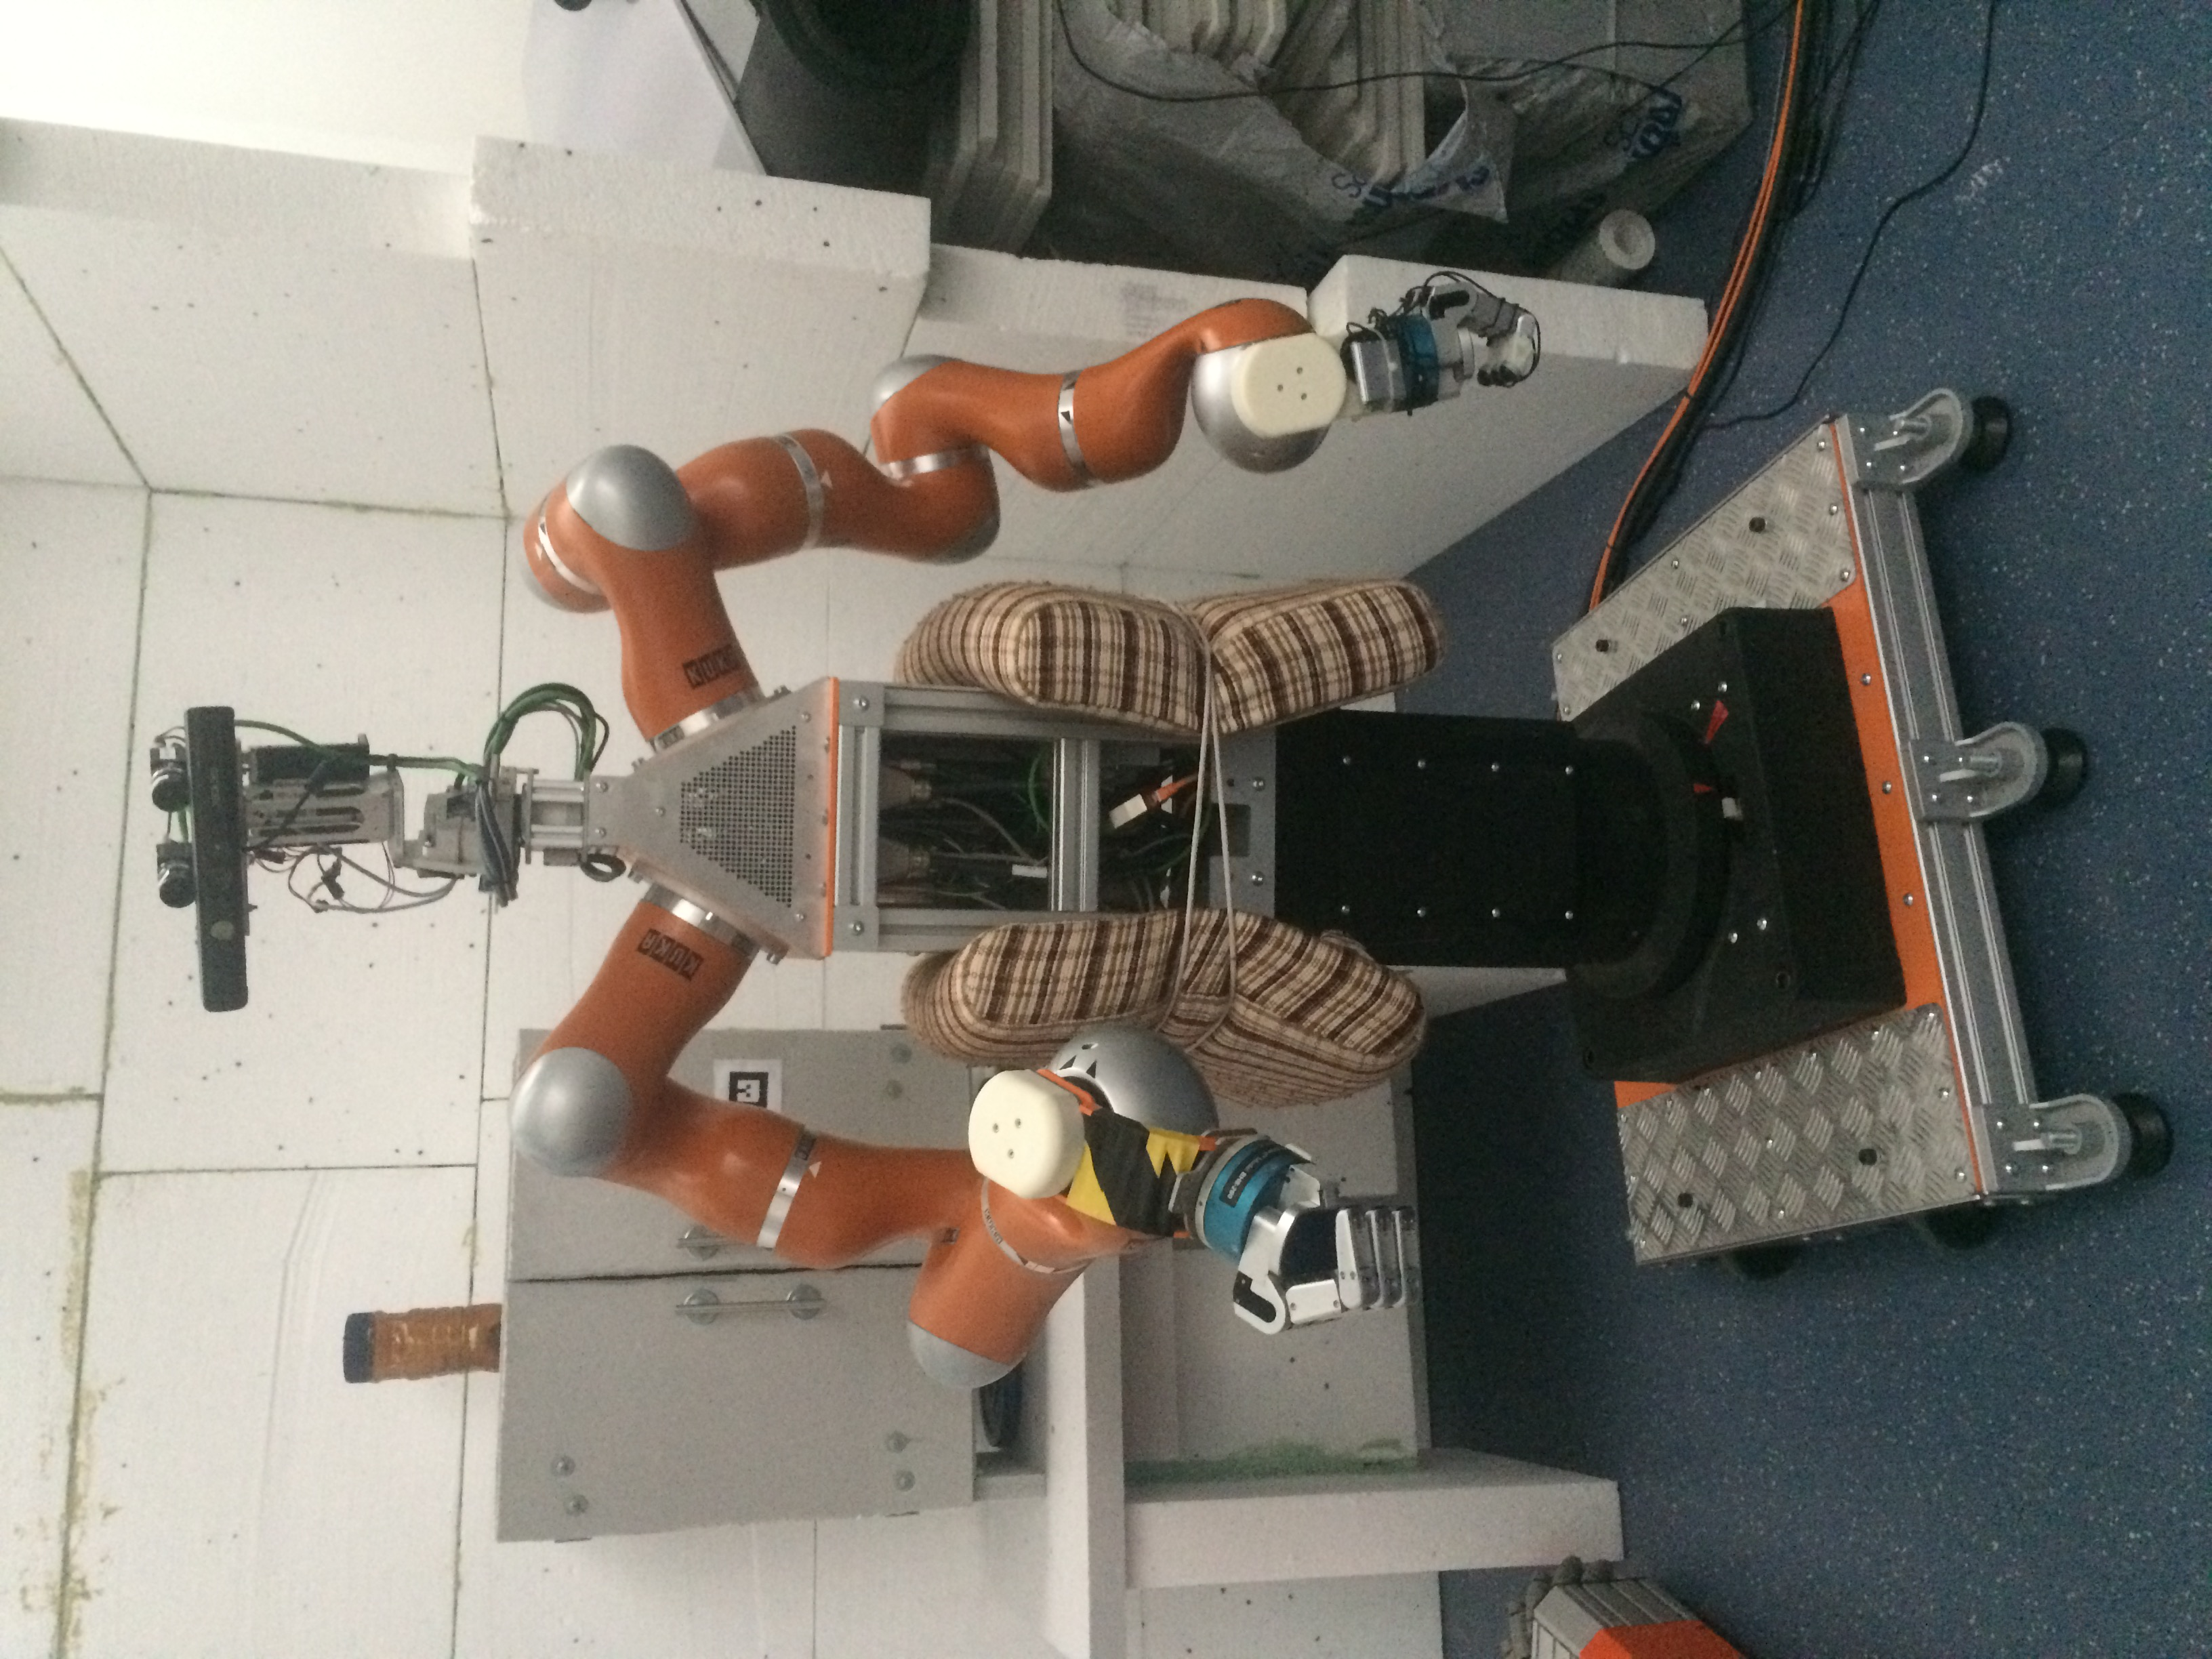
\includegraphics[scale=0.06, angle =-90]{velma1}
\end{figure}

\end{frame}

\begin{frame}{Struktura oprogramowania}

Struktura komponentowa. Częstotliwość pętli sterowania to 500 Hz.

\begin{itemize}
	\item ROS
	\item Orocos
\end{itemize}

Symulator działania z modelem fizyki i symulacją czasu.


\begin{itemize}
	\item Gazebo
	\item Dart
\end{itemize}
\end{frame}


\begin{frame}{Sterowanie ramieniem robota w obliczu chwytania przedmiotów}

\begin{itemize}
	\item Dr inż. Tomasz Winiarski
\end{itemize}

\begin{itemize}
	\item Sterowanie siłowe
	\item Odczyty wartości z efektorów i receptorów
	\item Nieznany model chwytanego obiektu
\end{itemize}
\end{frame}



\begin{frame}{Sterowanie impedancyjne}
	\begin{figure}[h]
		\centering
		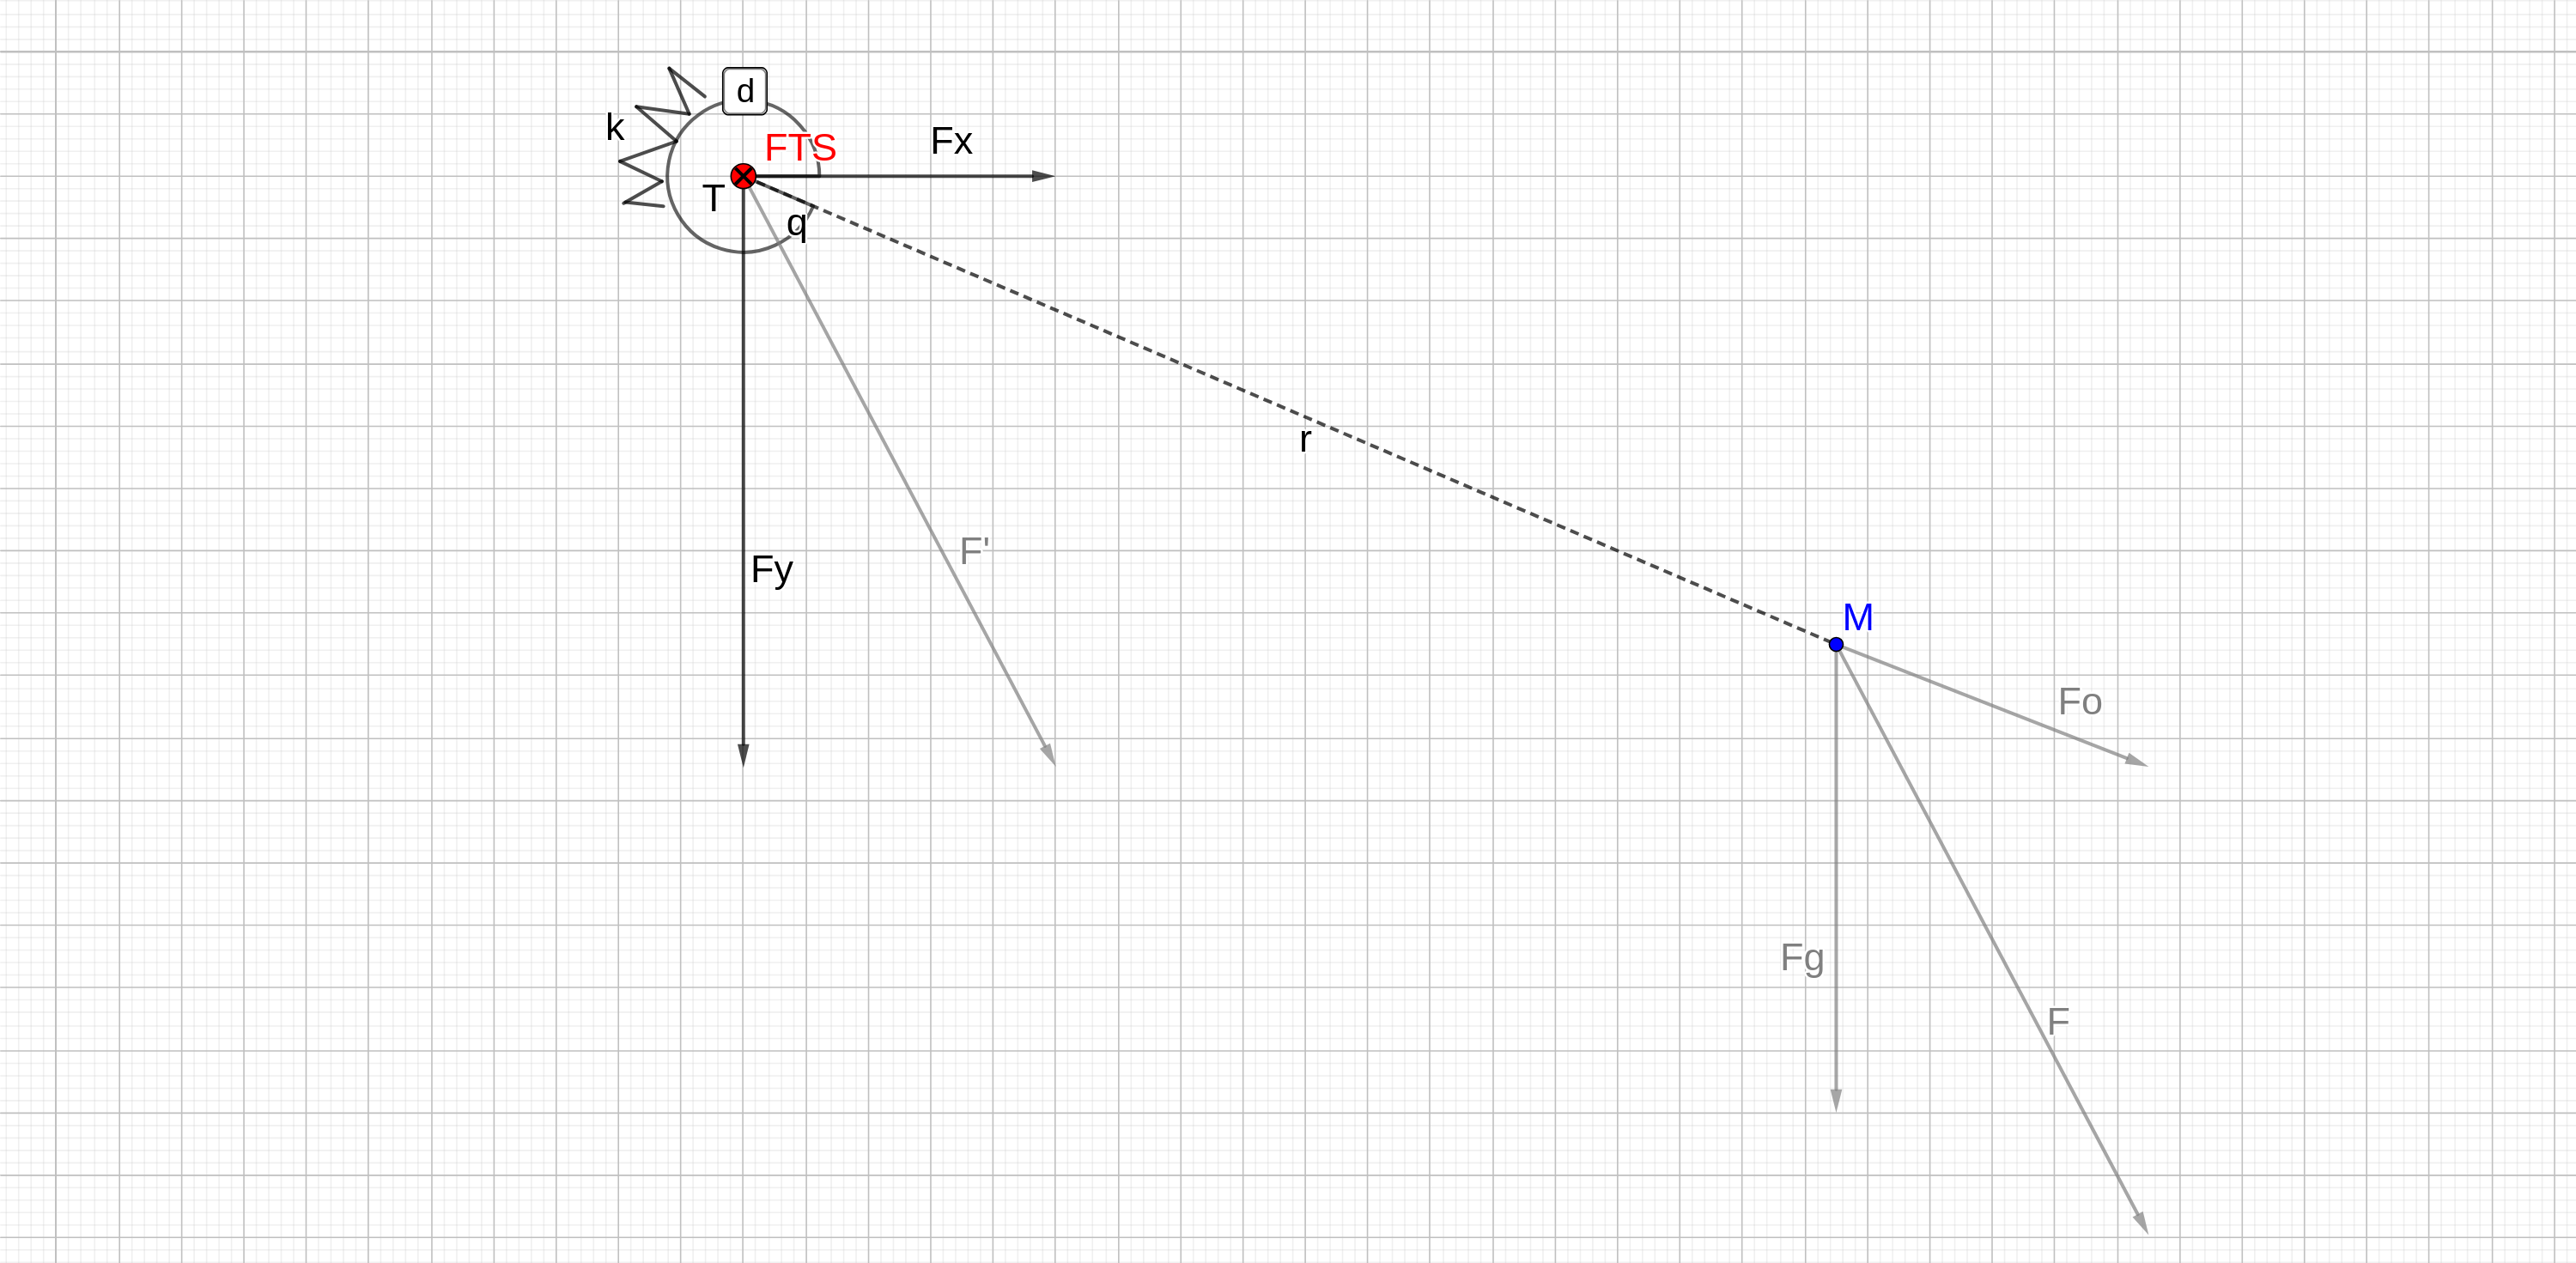
\includegraphics[scale=1.30]{2d}
	\end{figure}

	\begin{equation}
	\tau = K(q_d-q) + D(\dot{q}) + \hat{M}(q)\ddot{q_d} + \hat{c}(q, \dot{q}) + \hat{g}(q) + \hat{h}(q, \dot{q})
	\end{equation}
\end{frame}

\begin{frame}{Model obiektu}
\begin{itemize}
	\item Masa $m$
	\item Promień $R_{3x1}$
	\item Macierz inercji $I_{3x3}$
\end{itemize}
\end{frame}

\begin{frame}{Symulacja układu}
	Należy zastosować dyskretyzację równań.
	
\end{frame}

\begin{frame}{Parametry modelu}
\begin{equation}
F_i = ma_i
\end{equation}
\begin{equation}
\tau_i = M(q_i)\dot{\omega_i} + \omega_i \times M(q_i)\omega_i
\end{equation}

\end{frame}

\begin{frame}{Problem optymalizacji}

Można zastosować optymalizację minimalizującą sumę błędów kolejnych odczytów:
\begin{equation}
e_i = \begin{bmatrix}
F_i - \hat{F_i}\\
\tau_i - \hat{\tau_i} 
\end{bmatrix}
\end{equation}

\begin{equation}
\begin{aligned}
& \underset{m, r}{\text{min}}
& & \sum_{i = 1}^{n} || e_i ||
\end{aligned}
\end{equation}

\end{frame}


%\begin{frame}[allowframebreaks]{Bibliografia}
%\bibliographystyle{plain}
%\bibliography{bibliography}
%\end{frame}
\section{Podsumowanie}
\begin{frame}{Bibliografia}
Zdjęcia pochodzą ze strony \url{https://robotyka.ia.pw.edu.pl}
\end{frame}
\begin{frame}{Dziękuję za uwagę}
\begin{figure}[h]
	\centering
	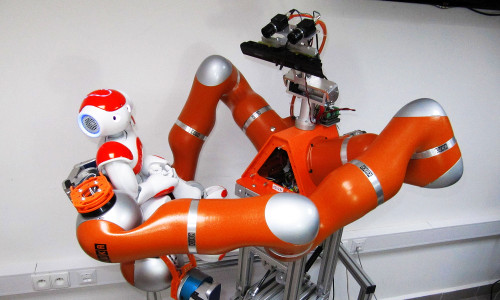
\includegraphics[scale=1.4]{velma3}
\end{figure}
\end{frame}
\end{document}